\documentclass[border=10pt]{standalone}

\usepackage{tikz}
\usepackage{tikzsymbols}
\usetikzlibrary{calc,patterns,shapes.geometric}

\def\centerarc[#1](#2)(#3:#4:#5){\draw[#1] ($(#2)+({#5*cos(#3)},{#5*sin(#3)})$) arc (#3:#4:#5);}

\begin{document}
	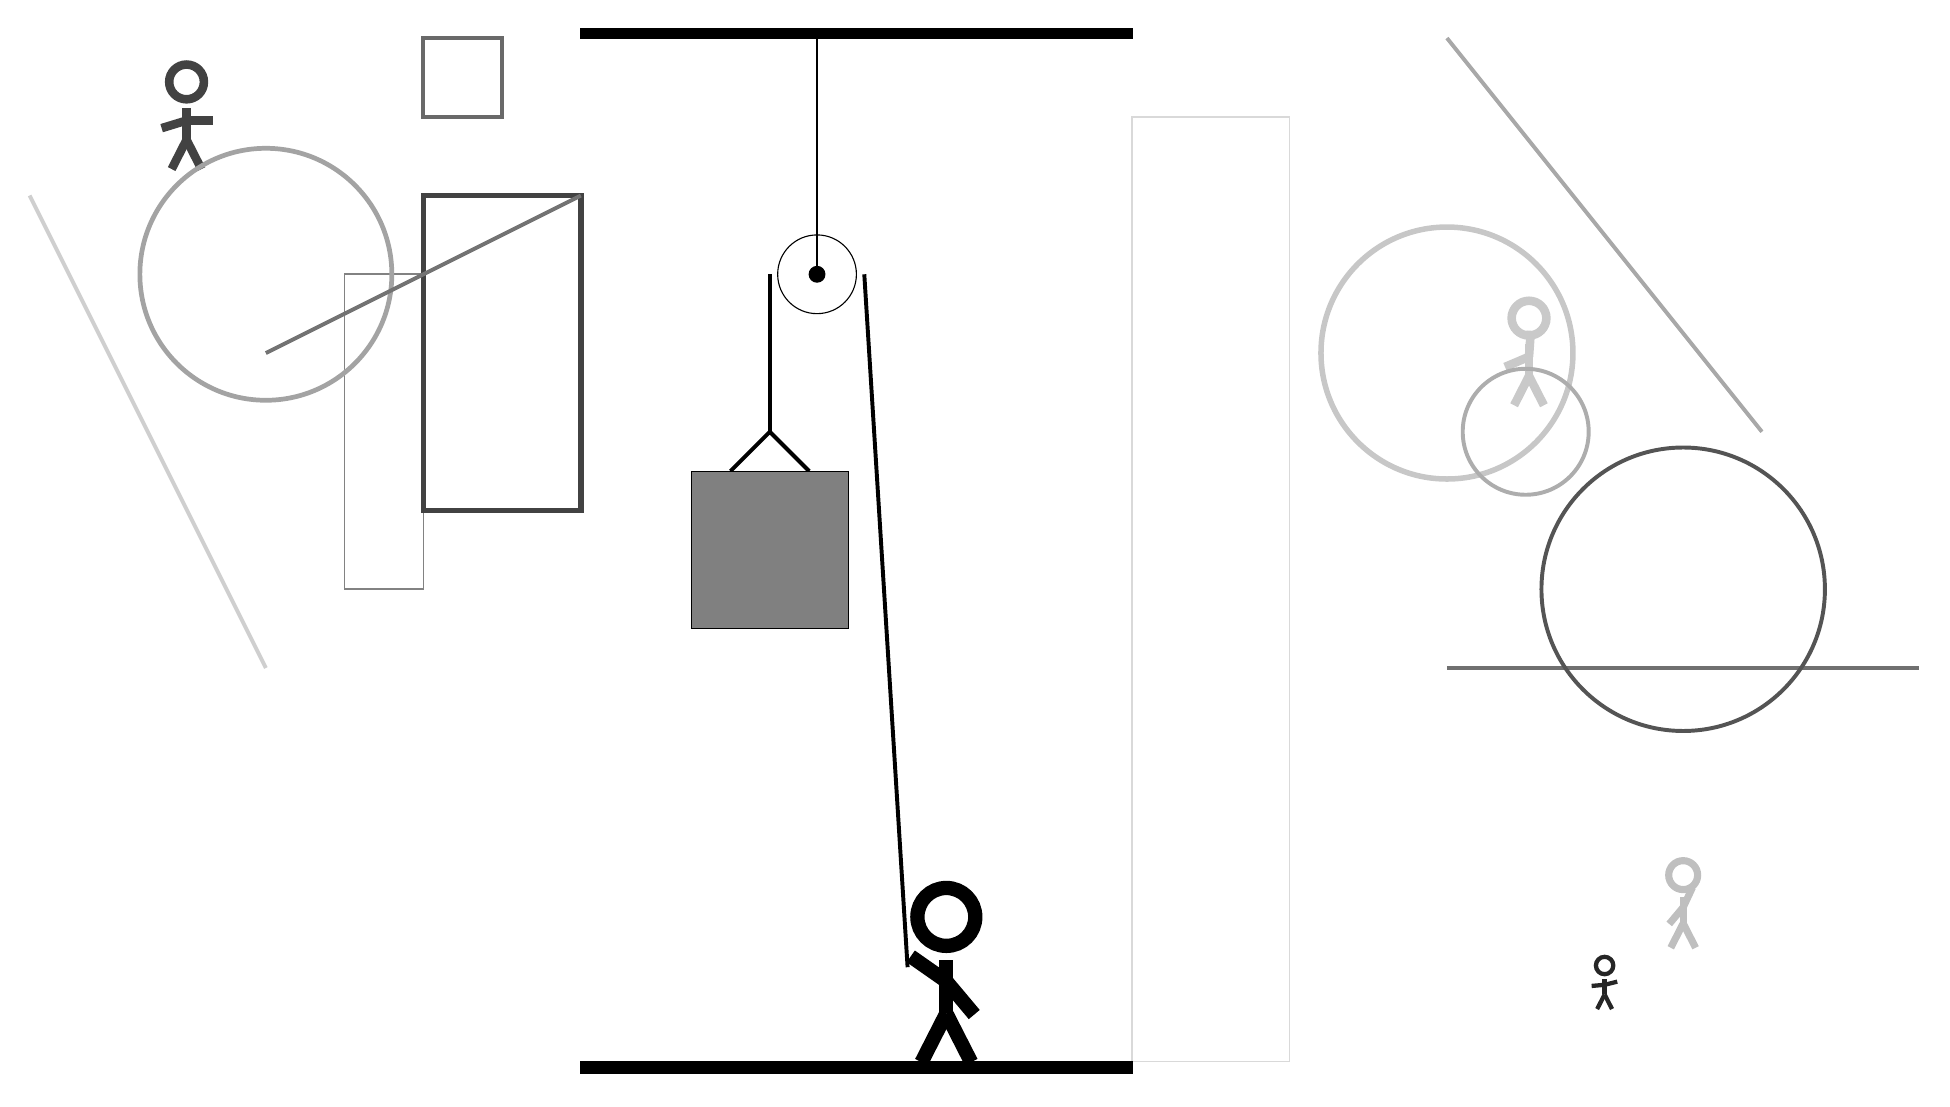
\begin{tikzpicture}
		%%%%% START %%%%%
		
		\draw[fill=black] (-2, 10) rectangle (5, 10.125);
		
		\draw (1, 7) circle (0.5);
		\draw[fill=black] (1, 7) circle (0.1);
		\draw (1, 10) -- (1, 7);
		
		\draw[line width=0.5mm] (-0.1, 4.5) -- (0.4, 5.0) -- (0.9, 4.5);
		\draw[fill=black!50] (-0.6, 4.5) rectangle (1.4, 2.5);
		
		\draw[line width=0.5mm] (0.4, 7) -- (0.4, 5.0);
		\centerarc[line width=0.5mm](1, 7)(0:180:0.6);
		\draw[line width=0.5mm](1.6, 7) -- (2.15, -1.8);
		
		\node at (2.6, -1.9) {\Strichmaxerl[10][-35][-50]};
		
		\draw[line width=0.2mm, color=black!49] (-4, 3) rectangle (-5, 7);
		
		\node[line width=0.5mm, color=black!74] at (-7, 9) {\Strichmaxerl[6][17][0]};
		\node[line width=0.6mm, color=black!85] at (11, -2) {\Strichmaxerl[3][5][14]};
		\draw [line width=0.6mm, color=black!36](-6, 7) circle (1.6);
		
		\draw[line width=0.5mm, color=black!19](-6, 2) -- (-9, 8);
		
		\node[line width=0.2mm, color=black!21] at (10, 6) {\Strichmaxerl[6][23][86]};
		\draw[line width=0.5mm, color=black!59] (-4, 10) rectangle (-3, 9);
		\node[line width=0.5mm, color=black!25] at (12, -1) {\Strichmaxerl[5][50][65]};
		\draw[line width=0.5mm, color=black!34](9, 10) -- (13, 5);
		\draw[line width=0.5mm, color=black!56](9, 2) -- (15, 2);
		\draw[line width=0.7mm, color=black!74] (-4, 4) rectangle (-2, 8);
		
		\draw[line width=0.2mm, color=black!15] (5, 9) rectangle (7, -3);
		\draw [line width=0.7mm, color=black!22](9, 6) circle (1.6);
		\draw[line width=0.5mm, color=black!55](-2, 8) -- (-6, 6);
		\draw [line width=0.5mm, color=black!67](12, 3) circle (1.8);
		\draw [line width=0.5mm, color=black!32](10, 5) circle (0.8);
		
		
		\draw[fill=black] (-2, -3) rectangle (5, -3.15);
		
		%%%%% END %%%%%
	\end{tikzpicture}
\end{document}